\subsection{Torque induced by the Static Field}
\label{sec:torqueBG}

Consider a metallic rigid cylinder shaped subject (a wire or rod) free to rotate, in a low friction surface, and align itself to a static magnetic field ($B_0$). The cylinder experiences a torque and has magnetic dipole moment according to eq. (\ref{eq:torque}). For a thin, linear paramagnetic material, the induced magnetic moment depends on its orientation relative to the static magnetic field. It can be expressed as

\begin{equation}
	\mathbf{m} = m_0 \cos (\theta),
	\label{eq:mprojection}
\end{equation}

\noindent where $m_0$ is the maximum induced dipole moment, which occurs when the material’s axis is aligned parallel to the $B_0$ field ($\theta$ = 0$^\circ$). When the material is oriented perpendicular to $B_0$ ($\theta$ = 90$^\circ$), the effective component of the dipole moment along the field direction vanishes. This follows from the projection of the dipole moment vector onto the magnetic field axis.

\begin{figure}[htb!]
	\centering
	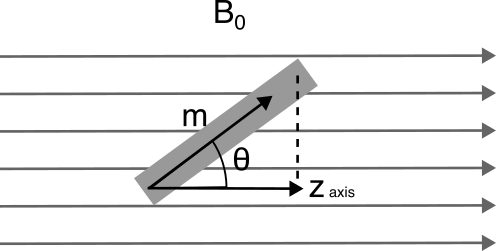
\includegraphics[width=0.65\textwidth]{Assets/dipole.png}
	\caption{Vector diagram of a magnetic dipole $\mathbf{m}$ in a uniform magnetic field $\mathbf{B}$ directed along the $z$-axis.}
	\label{fig:m0mcost}
\end{figure}

In Figure \ref{fig:m0mcost}, the dipole of length $a$, experiences a torque magnitude $|\boldsymbol{\tau}| = |\mathbf{m} \times \mathbf{B}| = m B_0 \sin\theta$. From the geometric projection of the dipole moment onto the magnetic field direction (eq. \ref{eq:mprojection}), and the torque experienced by the dipole we can write
\begin{equation*}
	|\boldsymbol{\tau}| = m_0 B_0 \sin(\theta) \cos(\theta) = m_0 B_0 \frac{\sin (2\theta)}{2}.
\end{equation*}

Using equation \ref{eq:magnitudemoment} for the dipole moment, we then write 

\begin{subequations}
	\begin{equation}
		\tau(\theta) = \tau_{max} \sin(2\theta), \text{or}
		\label{eq:torque_thetadependece}
	\end{equation}
	\begin{equation}
		\tau_{max} = \frac{\chi_m B_0^2 V}{2 \mu_0}.
		\label{eq:maxtorque}
	\end{equation}
	\label{eq:magnetic_torque}
\end{subequations}

Once the torque is found, a direct comparison to the body's weight can be made. According to ASTM F2213 \cite{astm2213, stoianovici2024}, the criterion ($c_\tau$) for evaluating magnetically induced torque on medical devices in a magnetic resonance environment is

\begin{equation}
	c_\tau = \frac{\tau_{max}}{mgL},
	\label{eq:gravTorque}
\end{equation} 

\noindent where $\tau_{max}$ is the maximum torque measured or obtained by equation \ref{eq:maxtorque}, meaning that the maximum magnetically induced torque is comparable than the product of the device's longest dimension ($L$) and its weight ($mg$). Under the ASTM gravity-based acceptability criterion, a device is considered acceptable when $c_\tau < 1$.